\section{Arsitektur Sistem}

\subsection{Diagram Arsitektur dan Diagram \textit{Deployment}}

Arsitektur Milestone 2 mempertahankan pemisahan peran layanan dari Milestone 1 lalu memperluasnya ke lingkungan klaster multi-\textit{node}. Seluruh alur masuk data dikendalikan oleh \textit{pod} Aggregator yang terkoordinasi, sementara jalur baca publik dilayani merata oleh seluruh replika melalui \texttt{client-api}. Aliran komponen logis beserta batas penyimpanannya diperlihatkan pada \textbf{Gambar~\ref{fig:m2-arch}}.

\begin{figure}[H]
  \centering
  \IfFileExists{figures/arsitektur-sistem-m2.png}{%
    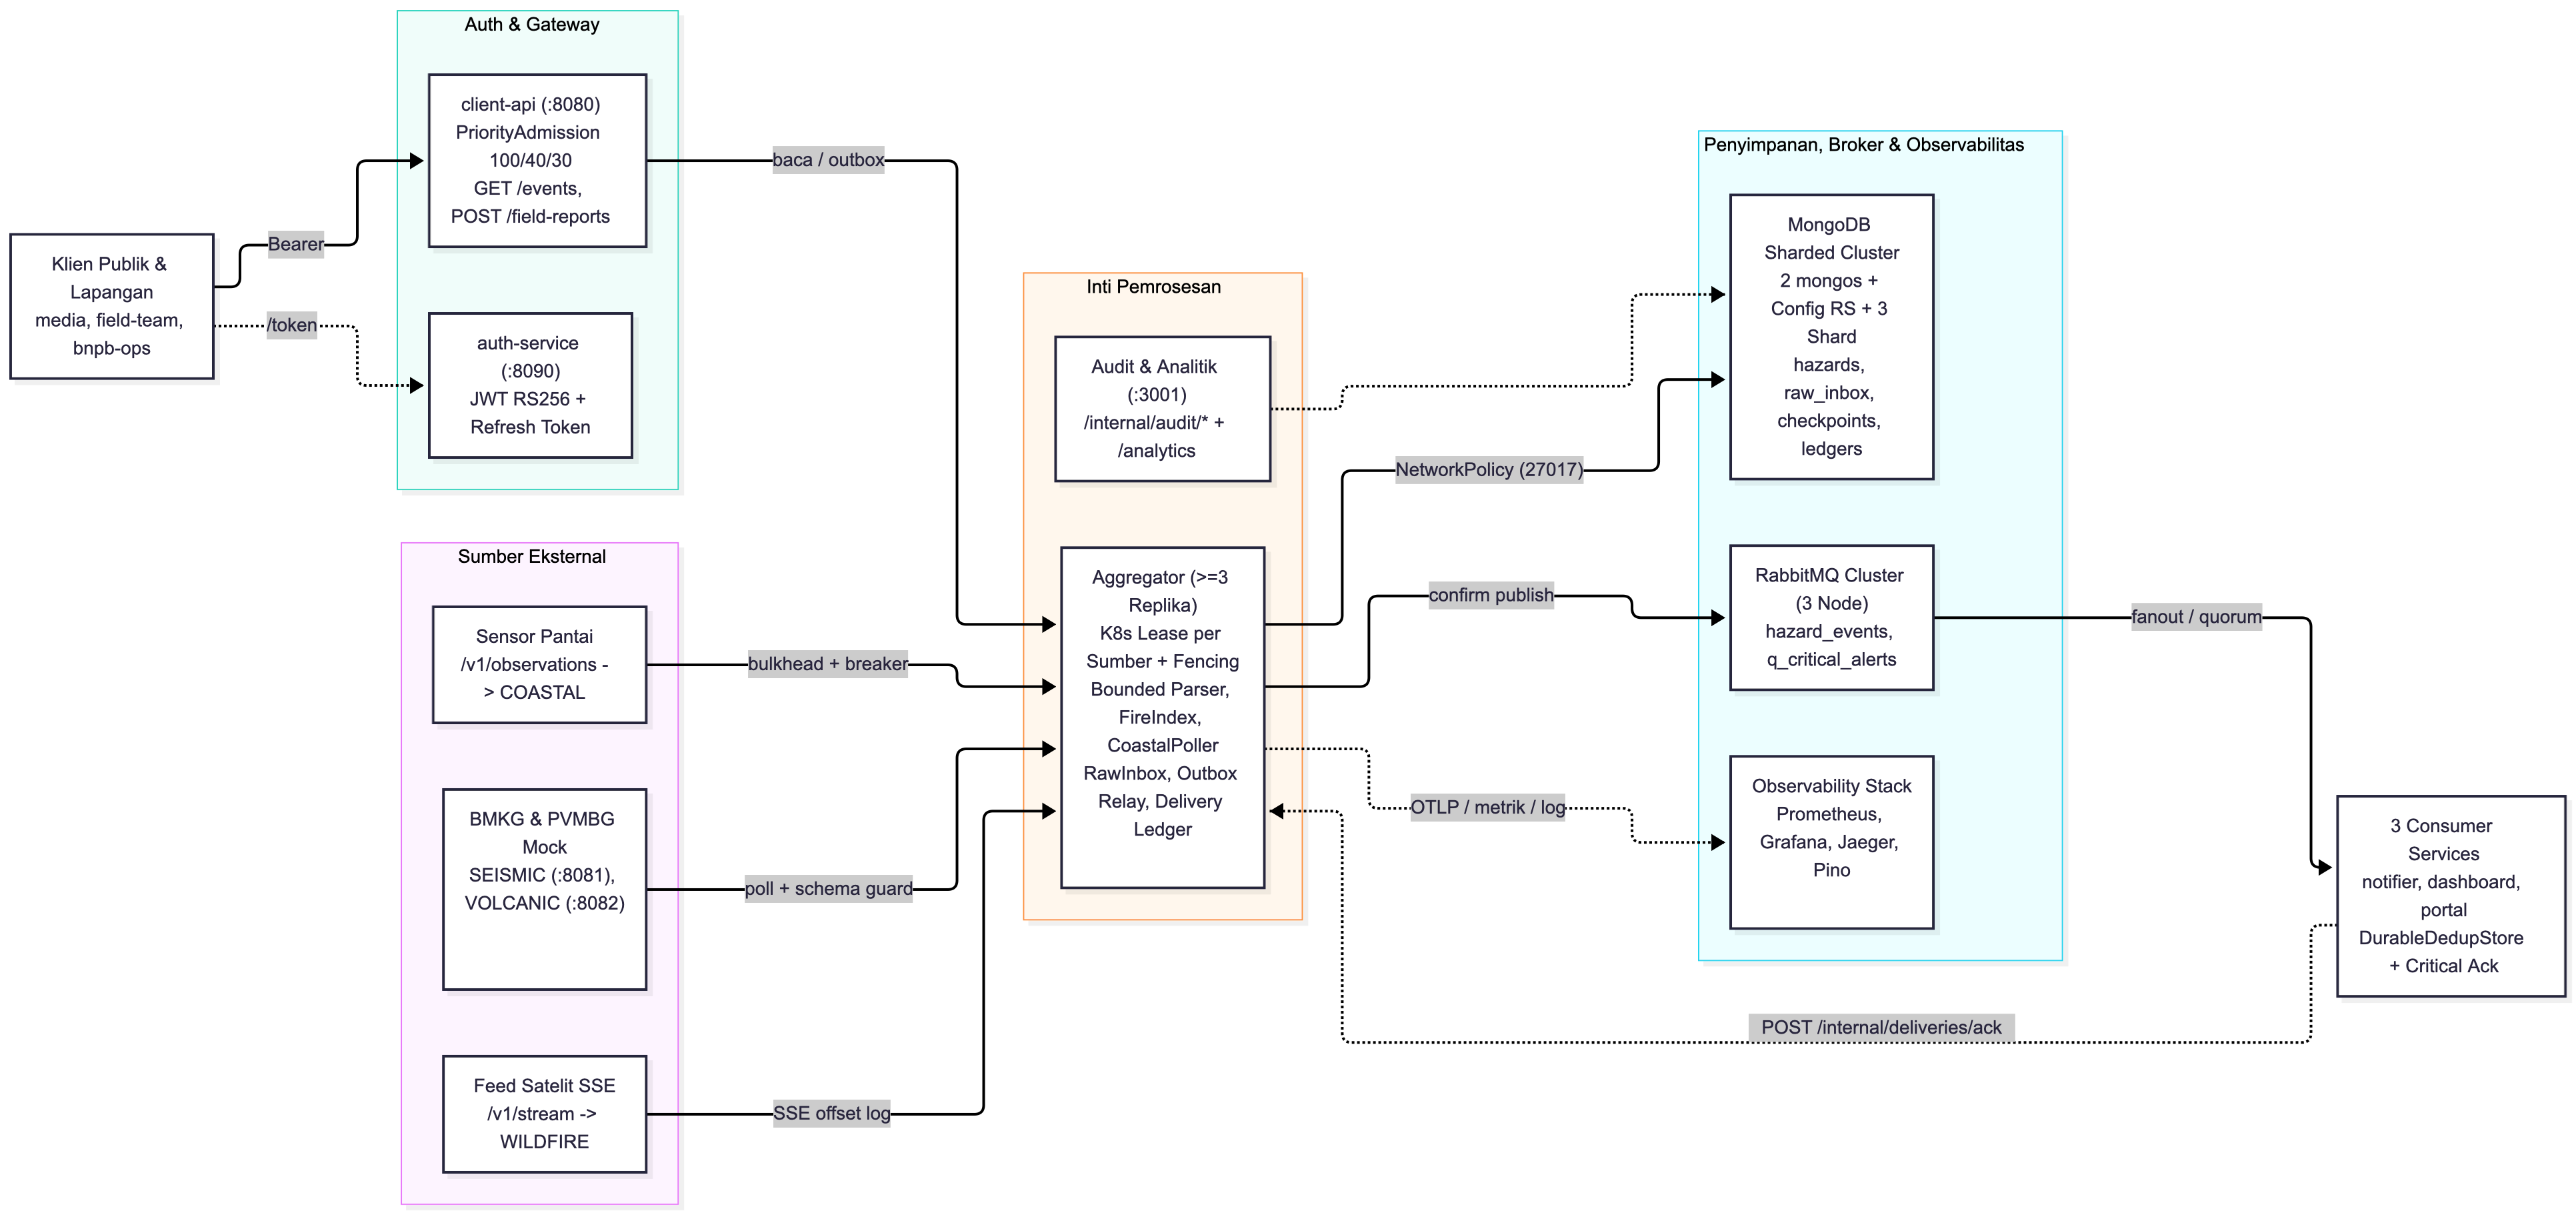
\includegraphics[width=0.96\linewidth]{arsitektur-sistem-m2.png}%
  }{%
  \resizebox{\linewidth}{!}{%
  \begin{tikzpicture}[
    every node/.style={font=\sffamily\footnotesize},
    box/.style={draw=black!65, rounded corners=3pt, fill=white, align=center, inner sep=5pt, minimum width=3.1cm, minimum height=0.88cm},
    store/.style={draw=blue!55!black, rounded corners=2pt, fill=blue!6, align=center, inner sep=5pt, minimum width=3.2cm, minimum height=0.88cm},
    obs/.style={draw=green!45!black, rounded corners=2pt, fill=green!5, align=center, inner sep=4.5pt, minimum width=3.1cm, minimum height=0.82cm},
    group/.style={draw=black!35, dashed, rounded corners=4pt, fill=black!2, inner sep=9pt},
    arr/.style={-{Stealth[length=2.2mm]}, thick, draw=black!75},
    lbl/.style={font=\sffamily\scriptsize, fill=white, inner sep=1.5pt, align=center}
  ]
    % Kolom 1: Sumber & Klien (x = 0)
    \node[box] (m1src) at (0, 5.4) {\textbf{BMKG \& PVMBG Mock}\\{\scriptsize SEISMIC (:8081), VOLCANIC (:8082)}};
    \node[box] (sat)   at (0, 3.6) {\textbf{Feed Satelit SSE}\\{\scriptsize /v1/stream $\to$ WILDFIRE}};
    \node[box] (coast) at (0, 1.8) {\textbf{Sensor Pantai}\\{\scriptsize /v1/observations $\to$ COASTAL}};
    \node[box] (cli)   at (0, 0.0) {\textbf{Klien Publik \& Lapangan}\\{\scriptsize media, field-team, bnpb-ops}};

    % Kolom 2: Auth & Gateway (x = 6.4)
    \node[box] (auth)  at (6.4, 1.6) {\textbf{auth-service (:8090)}\\{\scriptsize JWT RS256 + Refresh Token}};
    \node[box] (capi)  at (6.4, 0.0) {\textbf{client-api (:8080)}\\{\scriptsize PriorityAdmission 100/40/30}\\{\scriptsize GET /events, POST /field-reports}};

    % Kolom 3: Aggregator Terkoordinasi (x = 13.8)
    \node[box] (agg)   at (13.8, 3.4) {\textbf{Aggregator ($\ge$3 Replika)}\\{\scriptsize K8s Lease per Sumber + Fencing}\\{\scriptsize Bounded Parser, FireIndex, CoastalPoller}\\{\scriptsize RawInbox, Outbox Relay, Delivery Ledger}};
    \node[box] (audit) at (13.8, 0.2) {\textbf{Audit \& Analitik (:3001)}\\{\scriptsize /internal/audit/* + /analytics}};

    % Kolom 4: Storage & Broker (x = 21.2)
    \node[store] (mongo) at (21.2, 4.8) {\textbf{MongoDB Sharded Cluster}\\{\scriptsize 2 mongos + Config RS + 3 Shard}\\{\scriptsize hazards, raw\_inbox, checkpoints, ledgers}};
    \node[box]   (rmq)   at (21.2, 2.2) {\textbf{RabbitMQ Cluster (3 Node)}\\{\scriptsize hazard\_events, q\_critical\_alerts}};
    \node[obs]   (obsp)  at (21.2, 0.0) {\textbf{Observability Stack}\\{\scriptsize Prometheus, Grafana, Jaeger, Pino}};

    % Kolom 5: Consumers (x = 27.4)
    \node[box] (cons) at (27.4, 2.2) {\textbf{3 Consumer Services}\\{\scriptsize notifier, dashboard, portal}\\{\scriptsize DurableDedupStore + Critical Ack}};

    % Grouping
    \begin{scope}[on background layer]
      \node[group, fit=(m1src)(sat)(coast), label={[font=\sffamily\scriptsize\bfseries]above:Sumber Eksternal}] {};
      \node[group, fit=(agg)(audit), label={[font=\sffamily\scriptsize\bfseries]above:Inti Pemrosesan}] {};
    \end{scope}

    % Panah
    \draw[arr] (m1src.east) -- ++(1.1,0) |- node[lbl, pos=0.72, above] {poll + schema guard} ([yshift=7mm]agg.west);
    \draw[arr] (sat.east)   -- node[lbl, above] {SSE offset log} ([yshift=2mm]agg.west);
    \draw[arr] (coast.east) -- ++(1.1,0) |- node[lbl, pos=0.72, below] {bulkhead + breaker} ([yshift=-3mm]agg.west);

    \draw[arr] (cli) -- node[lbl, above] {Bearer} (capi);
    \draw[arr, dashed] ([yshift=2.5mm]cli.east) -- ++(0.9,0) |- node[lbl, pos=0.72, above] {/token} (auth.west);
    \draw[arr] (capi.east) -- ++(0.9,0) |- node[lbl, pos=0.72, below] {baca / outbox} ([yshift=-8mm]agg.west);

    \draw[arr] ([yshift=4mm]agg.east) -- ++(0.8,0) |- node[lbl, pos=0.72, above] {NetworkPolicy (27017)} (mongo.west);
    \draw[arr] ([yshift=-2mm]agg.east) -- ++(0.8,0) |- node[lbl, pos=0.72, above] {confirm publish} (rmq.west);
    \draw[arr] (rmq) -- node[lbl, above] {fanout / quorum} (cons);
    \draw[arr, dashed] (cons.south) -- ++(0,-3.1) -| node[lbl, pos=0.25, below] {POST /internal/deliveries/ack} ([xshift=6mm]agg.south);
    \draw[arr, dashed] (audit) -- (mongo.south west);
    \draw[arr, dashed] (agg.south east) |- (obsp.west);
  \end{tikzpicture}%
  }%
  }
  \caption{Diagram Arsitektur Logis Sistem Gateway Kebencanaan BNPB pada Milestone 2}
  \label{fig:m2-arch}
\end{figure}

Di tingkat infrastruktur, seluruh layanan dijalankan di atas tiga \textit{node} VM VirtualBox berkernel terpisah pada satu host fisik PC. Penempatan \textit{pod} per VM dan keterhubungan volume disk lokal diperlihatkan pada \textbf{Gambar~\ref{fig:m2-deploy}}.

\begin{figure}[H]
  \centering
  \IfFileExists{figures/deployment-cluster-m2.png}{%
    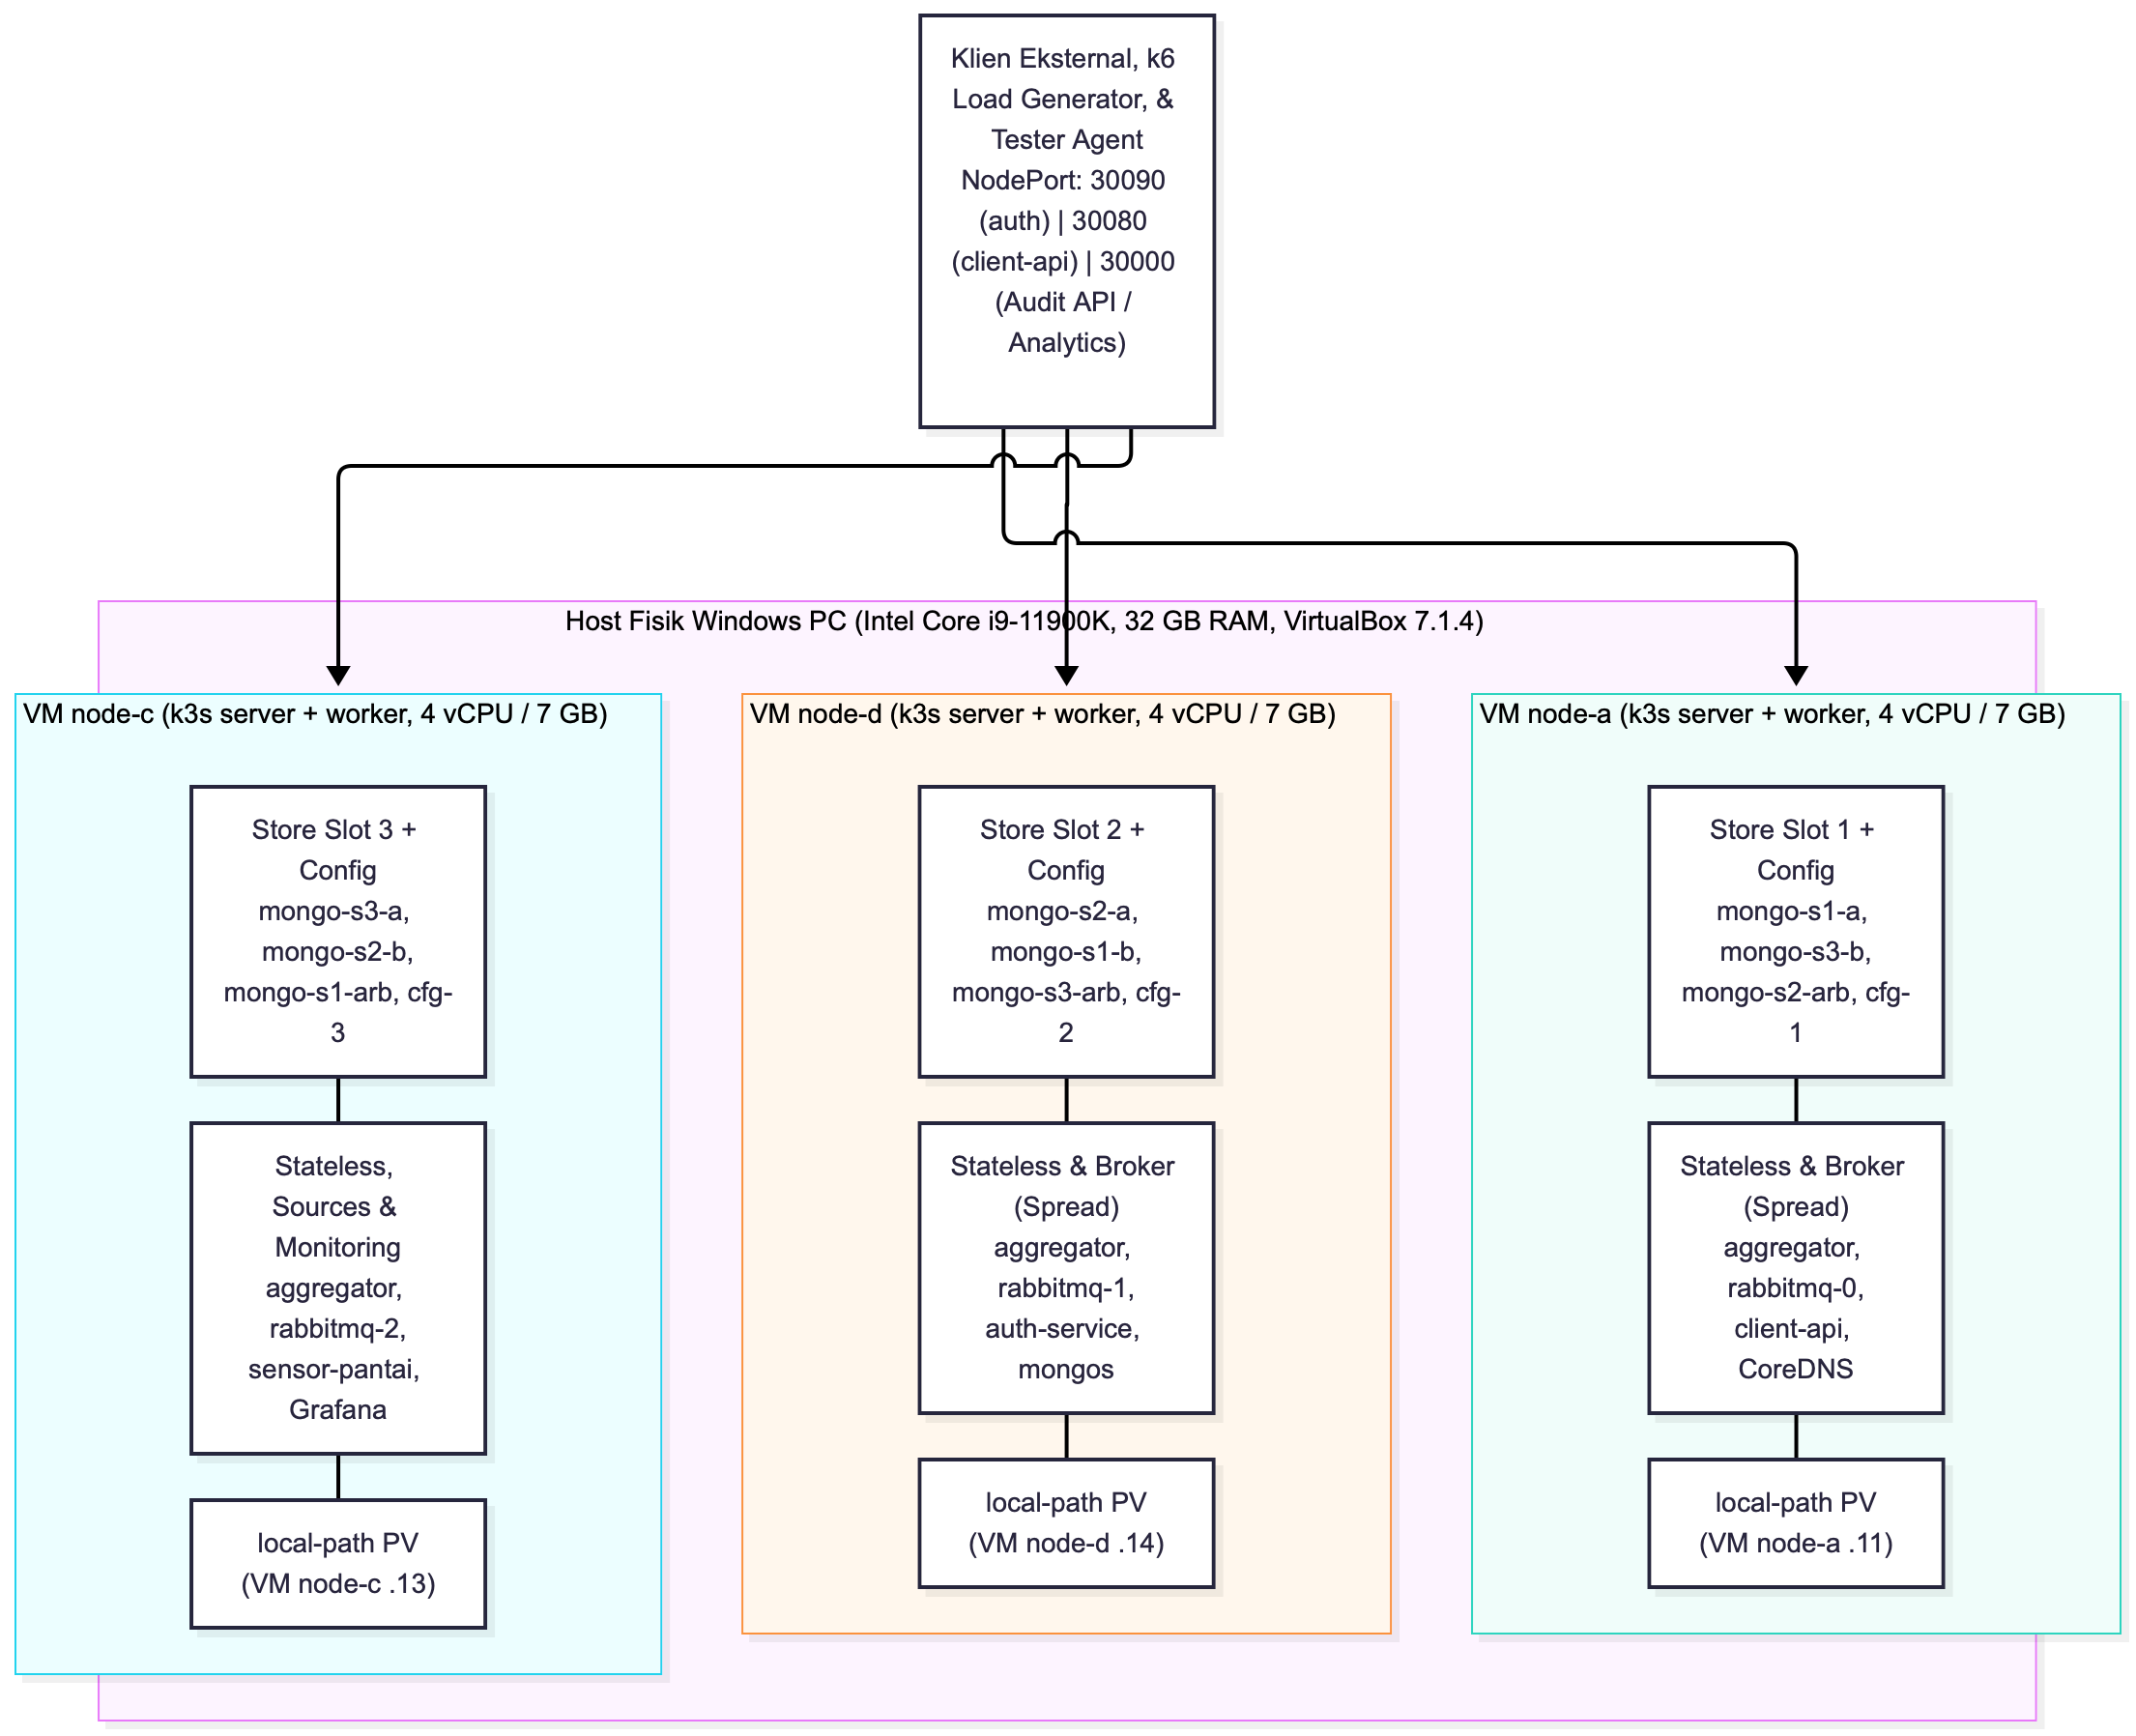
\includegraphics[width=0.96\linewidth]{deployment-cluster-m2.png}%
  }{%
  \resizebox{\linewidth}{!}{%
  \begin{tikzpicture}[
    every node/.style={font=\sffamily\footnotesize},
    pod/.style={draw=black!65, rounded corners=2pt, fill=white, align=center, inner sep=4pt, minimum width=4.8cm, minimum height=0.75cm},
    pv/.style={draw=blue!55!black, rounded corners=2pt, fill=blue!6, align=center, inner sep=4pt, minimum width=4.8cm, minimum height=0.58cm},
    vm/.style={draw=black!45, dashed, rounded corners=4pt, fill=black!2, inner sep=8pt},
    host/.style={draw=black!65, rounded corners=5pt, fill=black!1, inner sep=12pt},
    arr/.style={-{Stealth[length=2mm]}, thick, draw=black!70},
    lbl/.style={font=\sffamily\scriptsize, fill=white, inner sep=1.5pt}
  ]
    % Node A
    \node[pod] (a1) at (0, 3.0) {\textbf{Store Slot 1 + Config}\\{\scriptsize mongo-s1-a, mongo-s3-b, mongo-s2-arb, cfg-1}};
    \node[pod] (a2) at (0, 2.0) {\textbf{Stateless \& Broker (Spread)}\\{\scriptsize aggregator, rabbitmq-0, client-api, CoreDNS}};
    \node[pv]  (a3) at (0, 1.0) {\scriptsize local-path PV (VM node-a $\cdot$ .11)};

    % Node D (Slot 2)
    \node[pod] (d1) at (6.5, 3.0) {\textbf{Store Slot 2 + Config}\\{\scriptsize mongo-s2-a, mongo-s1-b, mongo-s3-arb, cfg-2}};
    \node[pod] (d2) at (6.5, 2.0) {\textbf{Stateless \& Broker (Spread)}\\{\scriptsize aggregator, rabbitmq-1, auth-service, mongos}};
    \node[pv]  (d3) at (6.5, 1.0) {\scriptsize local-path PV (VM node-d $\cdot$ .14)};

    % Node C (Slot 3)
    \node[pod] (c1) at (13.0, 3.0) {\textbf{Store Slot 3 + Config}\\{\scriptsize mongo-s3-a, mongo-s2-b, mongo-s1-arb, cfg-3}};
    \node[pod] (c2) at (13.0, 2.0) {\textbf{Stateless, Sources \& Monitoring}\\{\scriptsize aggregator, rabbitmq-2, sensor-pantai, Grafana}};
    \node[pv]  (c3) at (13.0, 1.0) {\scriptsize local-path PV (VM node-c $\cdot$ .13)};

    % VM boxes & Host box
    \begin{scope}[on background layer]
      \node[vm, fit=(a1)(a2)(a3), label={[font=\sffamily\scriptsize\bfseries]above:VM node-a (k3s server + worker, 4 vCPU / 7 GB)}] (va) {};
      \node[vm, fit=(d1)(d2)(d3), label={[font=\sffamily\scriptsize\bfseries]above:VM node-d (k3s server + worker, 4 vCPU / 7 GB)}] (vd) {};
      \node[vm, fit=(c1)(c2)(c3), label={[font=\sffamily\scriptsize\bfseries]above:VM node-c (k3s server + worker, 4 vCPU / 7 GB)}] (vc) {};
      \node[host, fit=(va)(vd)(vc), label={[font=\sffamily\footnotesize\bfseries]above:Host Fisik Windows PC (Intel Core i9-11900K, 32 GB RAM, VirtualBox 7.1.4)}] {};
    \end{scope}

    % External Entry
    \node[pod, minimum width=9.5cm] (ext) at (6.5, -0.7) {\textbf{Klien Eksternal, k6 Load Generator, \& Tester Agent}\\{\scriptsize NodePort: 30090 (auth) $\cdot$ 30080 (client-api) $\cdot$ 30000 (Audit API / Analytics)}};
    \draw[arr] (ext.north) -- (a3.south);
    \draw[arr] (ext.north) -- (d3.south);
    \draw[arr] (ext.north) -- (c3.south);
  \end{tikzpicture}%
  }%
  }
  \caption{Diagram \textit{Deployment} Antar-\textit{Node} Klaster Kubernetes pada Tiga Mesin Virtual}
  \label{fig:m2-deploy}
\end{figure}

Setiap VM di dalam klaster juga menjalankan satu \textit{pod} \texttt{tester-agent} melalui \textit{DaemonSet} resmi serta komponen sistem pendukung seperti \textit{CoreDNS} (3 replika), \textit{local-path-provisioner} (2 replika), dan \textit{metrics-server} (2 replika). Pembagian posisi ini memastikan layanan penemuan DNS dan pencatatan volume tetap bertahan saat salah satu VM dimatikan paksa.

\subsection{Deklarasi Topologi}

Seluruh komponen aplikasi BNPB dijalankan pada klaster tiga VM di atas satu mesin host fisik dengan spesifikasi yang tercantum pada \textbf{Tabel~\ref{tab:topo-decl}}. Pada awal pengujian klaster terdapat \texttt{node-b} yang kemudian digantikan oleh \texttt{node-d} melalui skenario kehilangan \textit{node} Problem 1.

\begin{table}[H]
  \centering
  \caption{Deklarasi Topologi \textit{Node} Klaster Milestone 2}
  \label{tab:topo-decl}
  \small
  \begin{tabularx}{\linewidth}{@{} >{\raggedright\arraybackslash}p{1.8cm} >{\raggedright\arraybackslash}p{2.9cm} >{\raggedright\arraybackslash}p{2.5cm} >{\raggedright\arraybackslash}p{3.0cm} >{\raggedright\arraybackslash}X @{}}
    \toprule
    \textbf{Nama \textit{Node}} & \textbf{Peran K8s} & \textbf{Jenis \textit{Node}} & \textbf{Host \& VM} & \textbf{Komponen Utama} \\
    \midrule
    \texttt{node-a} (.11) & \textit{control-plane}, \textit{etcd}, \textit{worker} & VM (\textit{VirtualBox 7.1.4}) & PC Windows i9-11900K 32 GB, VM 4 vCPU / 7 GB & Slot 1 (\texttt{s1-a}, \texttt{s3-b}, \texttt{s2-arb}, \texttt{cfg-1}), \texttt{aggregator}, \texttt{rabbitmq-0} \\
    \midrule
    \texttt{node-d} (.14) & \textit{control-plane}, \textit{etcd}, \textit{worker} & VM (\textit{VirtualBox 7.1.4}) & Host PC sama, VM 4 vCPU / 7 GB & Slot 2 (\texttt{s2-a}, \texttt{s1-b}, \texttt{s3-arb}, \texttt{cfg-2}), \texttt{aggregator}, \texttt{rabbitmq-1} \\
    \midrule
    \texttt{node-c} (.13) & \textit{control-plane}, \textit{etcd}, \textit{worker} & VM (\textit{VirtualBox 7.1.4}) & Host PC sama, VM 4 vCPU / 7 GB & Slot 3 (\texttt{s3-a}, \texttt{s2-b}, \texttt{s1-arb}, \texttt{cfg-3}), \texttt{aggregator}, \texttt{rabbitmq-2} \\
    \bottomrule
  \end{tabularx}
\end{table}

Berdasarkan deklarasi sumber daya Lampiran B, total permintaan memori kondisi stabil (\textit{steady state}) seluruh \textit{pod} tercatat sekitar \texttt{10.624 Mi} (\texttt{10,4 Gi}) dengan batas maksimal \texttt{21.248 Mi}. Setiap VM berkapasitas \texttt{7 GB RAM} menanggung sekitar \texttt{3,5 Gi} permintaan \textit{pod} ditambah \texttt{1 Gi} kebutuhan sistem operasi dan \textit{k3s}. Pengukuran aktual di atas klaster dengan lebih dari 70.000 catatan menunjukkan pemakaian riil hanya \texttt{1,9 GiB} total atau $16$--$32\%$ RAM per \textit{node}.

\subsection{Pemilihan Teknologi dan Perubahan Kontrak}

Pemilihan teknologi pada Milestone 2 menekankan kompatibilitas penuh dengan Milestone 1, efisiensi memori kontainer, serta dukungan pemulihan otomatis saat terjadi kegagalan fisik. \textbf{Tabel~\ref{tab:m2-tech}} merangkum teknologi yang dipilih untuk tiap lapisan komponen beserta alasannya.

\begin{table}[H]
  \centering
  \caption{Teknologi Terpilih dan Alasan Pemilihannya pada Milestone 2}
  \label{tab:m2-tech}
  \small
  \begin{tabularx}{\linewidth}{@{} >{\raggedright\arraybackslash}p{3.2cm} >{\raggedright\arraybackslash}p{3.8cm} >{\raggedright\arraybackslash}X @{}}
    \toprule
    \textbf{Komponen} & \textbf{Teknologi} & \textbf{Alasan Pemilihan} \\
    \midrule
    Orkestrasi Klaster & Kubernetes (\textit{k3s}) multi-VM & Ringan dijalankan pada tiga VM \texttt{7 GB}, mendukung \textit{StatefulSet}, \textit{ConfigMap}, \textit{Secret}, \textit{NetworkPolicy}, serta objek \texttt{Lease} bawaan untuk pemilihan pemimpin. \\
    \midrule
    Penyimpanan Kanonik & MongoDB \texttt{4.4.30 Sharded Cluster} & Mendukung \textit{hashed sharding} dan rotasi replika di atas disk lokal VM. Versi \texttt{4.4.30} dipakai karena VM tamu VirtualBox tidak mengekspos instruksi CPU AVX milik MongoDB 5 ke atas. \\
    \midrule
    \textit{Message Broker} & RabbitMQ klaster 3-\textit{node} dengan \textit{quorum queue} & Menjaga pesan antrean kritis \path{q_critical_alerts} tidak hilang ketika satu VM maupun \textit{pod broker} mati mendadak. \\
    \midrule
    Layanan Aplikasi & Node.js + TypeScript + Express & Konsisten dengan basis kode Milestone 1 dan ringan secara memori (\texttt{256Mi}--\texttt{512Mi} per \textit{pod}) untuk pemrosesan asinkron berkecepatan tinggi. \\
    \midrule
    Observabilitas dan Uji & Prometheus, Grafana, Jaeger, Pino, dan \texttt{k6} & Menggabungkan pemantauan metrik waktu nyata, pelacakan \textit{span} terdistribusi, log terstruktur, dan pengujian beban terukur dari luar klaster. \\
    \bottomrule
  \end{tabularx}
\end{table}

Dari sisi kontrak data dan antarmuka, Milestone 2 menambahkan perluasan kompatibel tanpa merusak klien Milestone 1. Jenis bahaya kini meliputi \texttt{WILDFIRE} dari sumber \texttt{SATELIT} dan \texttt{COASTAL} dari sumber \texttt{SENSOR\_PANTAI}, serta asal laporan lapangan \texttt{FIELD\_REPORT}.

Pada API publik \texttt{client-api}, tersedia \texttt{POST} \path{/field-reports} berbalasan \texttt{202 Accepted} dengan pengaman \texttt{Idempotency-Key} serta jalur pemeriksaan pesan gagal \texttt{GET} \path{/unprocessed*} khusus bagi peran \texttt{bnpb-ops}. Respons \texttt{GET} \path{/events} tetap memakai format Milestone 1 pada kondisi normal, dan hanya menyertakan properti \texttt{partial: true}, daftar \texttt{unavailable\_units}, serta status kesegaran \texttt{sources.SENSOR\_PANTAI.stale} ketika terjadi gangguan.

\subsection{Observabilitas dan Audit API}

Ketiga pilar observabilitas dipasang pada \textit{namespace} \texttt{sistem-\allowbreak informasi-\allowbreak kebencanaan-\allowbreak bnpb} (\path{docs/m2-details/observability.md}):

\begin{enumerate}
  \item \textbf{Metrik terpadu (Prometheus dan Grafana):} Prometheus menyapu otomatis seluruh 21 target \textit{pod} aktif (meliputi layanan inti, \textit{mock}, pengekspor RabbitMQ pada port \texttt{15692}, tiga pengekspor MongoDB per \textit{shard}, serta \textit{cAdvisor}). Data disajikan ke dalam empat dasbor Grafana yang sudah terpasang otomatis: ringkasan BNPB, koordinasi dan \textit{store}, aliran satelit Problem 4, serta ketahanan pantai Problem 5.
  \item \textbf{Jejak terdistribusi (OpenTelemetry ke Jaeger):} layanan \texttt{client-api}, \texttt{aggregator}, dan ketiga \textit{consumer} mengirimkan \textit{span} lewat OTLP/HTTP ke \path{http://jaeger:4318} dengan membawa \textit{header} \texttt{traceparent}. Karena \textit{mock}, MongoDB, RabbitMQ, dan \textit{image} sensor tidak memancarkan \textit{span}, kesinambungan jejak melintasi \textit{broker} ditautkan lewat atribut \texttt{correlation\_id} dan kolom \texttt{traceparent}.
  \item \textbf{Log terstruktur (Pino JSON):} setiap baris log memuat \texttt{correlation\_id}, \texttt{trace\_id}, \texttt{service}, \texttt{pod}, \texttt{node}, \texttt{duration\_ms}, dan \texttt{error\_code} untuk investigasi insiden antarlayanan.
\end{enumerate}

Untuk verifikasi independen saat pengujian, Aggregator menyediakan \textbf{Audit API} sesuai Lampiran A pada jalur \path{/internal/audit/*} (\path{aggregator/src/storage/routes.ts}). Seluruh akses wajib menyertakan token internal khusus auditor dan mencakup empat \textit{endpoint} utama berikut:

\begin{itemize}
  \item \texttt{GET} \path{/internal/audit/events}: mengembalikan daftar \texttt{HazardEvent} kanonik berurutan waktu masuk (\texttt{ingested\_at asc}) dengan \textit{keyset cursor} serta penanda \texttt{partial}.
  \item \texttt{GET} \path{/internal/audit/checksum}: menghitung \textit{hash} SHA-256 atas \texttt{source\_\allowbreak ref\_id} terurut sebagai pembanding keutuhan data terhadap referensi penguji.
  \item \texttt{GET} \path{/internal/audit/location}: memeriksa anggota data aktif per \textit{shard} untuk melaporkan lokasi \textit{pod} dan \textit{node} VM penyimpanan tiap \texttt{hazard\_id}.
  \item \texttt{GET} \path{/internal/audit/unprocessed}: menampilkan daftar pesan berstatus \texttt{retrying} atau \texttt{parked} dari koleksi \path{raw_inbox}.
\end{itemize}

\subsection{Petunjuk Menjalankan Sistem}

Seluruh sistem disiapkan agar dapat dijalankan dari kondisi awal klaster kosong melalui satu perintah \textit{deploy} berbasis skrip \path{scripts/m2/deploy.sh}. Langkah operasionalnya meliputi tiga tahap berikut.

\begin{enumerate}
  \item \textbf{Siapkan berkas kredensial dan rahasia acak:} salin templat lingkungan lalu bangkitkan token dan kata sandi menggunakan skrip pembantu di akar repositori.
  \item \textbf{Persiapkan label \textit{node} dan \textit{image} (khusus klaster \textit{demo} multi-VM):} pasang label slot penyimpanan \texttt{1..3} pada ketiga VM via \path{scripts/m2/label-nodes.sh}, lalu bangun dan unggah \textit{image} ke registri yang dapat diakses oleh ketiga \textit{node}.
  \item \textbf{Jalankan perintah \textit{deploy} tunggal dan verifikasi dasar:} jalankan skrip deployment untuk \textit{overlay} \texttt{demo} (atau \texttt{dev} untuk klaster \textit{kind} lokal), lalu periksa sumber daya, fungsionalitas dasar, dan isolasi jaringan.
\end{enumerate}

\begin{lstlisting}[language=bash]
# 1. Siapkan kredensial lokal (.env)
cp .env.example .env && ./scripts/m1/gen-secrets.sh >> .env

# 2. (Mode demo 3-VM) Beri label node slot dan unggah image
./scripts/m2/label-nodes.sh node-a node-b node-c
PUSH=1 REGISTRY=<alamat-registry> TAG=demo ./scripts/m2/build-images.sh

# 3. Satu perintah deploy penuh + verifikasi awal (selaras README.md)
REGISTRY=<alamat-registry> ./scripts/m2/deploy.sh demo
./scripts/m2/verify-resources.sh && ./scripts/m2/smoke.sh && ./scripts/m2/verify-isolation.sh
\end{lstlisting}
